\chapter{Systemarkitektur}\label{Systemarkitektur}
Der er udarbejdet forskellige diagrammer på baggrund af de specificerede systemkrav. Diagrammerne har til formål at dele systemet op i realiserbare dele for at vise arkitekturen for og designet af Automatisk Ultralydsscanner. 

Arkitekturen beskriver den grundlæggende organisering af Automatisk Ultralydsscanner og opbygningen af dens tilhørende PC Applikation. Automatisk Ultralydsscanner er opbygget generisk, så man vil kunne udskifte komponenter som f.eks. Robotarm eller 3D kamera med en anden type. Det vil dog resultere i en anderledes implementering. Der er i diagrammerne designet ud fra, at 3D kamera er af typen Kinect 2.0 og Robotarm er en UR10 robot. 

Nedenfor vil relevante diagrammer blive gennemgået. For detaljeret gennemgang af systemarkitektur for Automatisk Ultralydsscanner se Bilag  \ref{Udviklingsdokument} Udviklingsdokument

\section{Domænemodel}
Nedenstående domænemodel Figur \ref{domain} udgør den overordnede systemarkitektur og tydeliggør forbindelserne og interaktionerne mellem de forskellige aktører i Automatisk Ultralydsscanner. 

\begin{figure}[H]
    \centering
    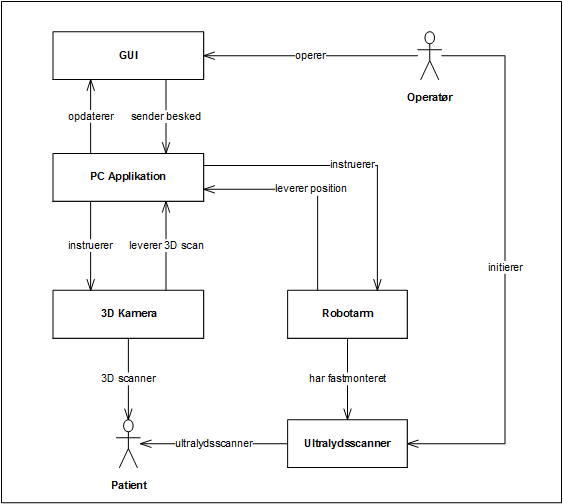
\includegraphics[width=0.7\textwidth]{figurer/d/Design/uml_domain}
    \caption{Domænemodel for Automatisk Ultralydsscanner}
    \label{domain}
\end{figure}

\section{Block definition diagram}
Automatisk Ultralydsscanner består af Robotarm, en computer, et Access Point, 3D kamera og Ultralydsscanner. Det er vigtigt at bemærke, at computer skal have PC Applikationen installeret og en mus og en skærm for at Operatør kan intergere med PC Applikation. Block Definitions diagrammet viser Figur \ref{BDD}, hvordan systemets blokke er forbundet. 

\begin{figure}[H]
    \centering
    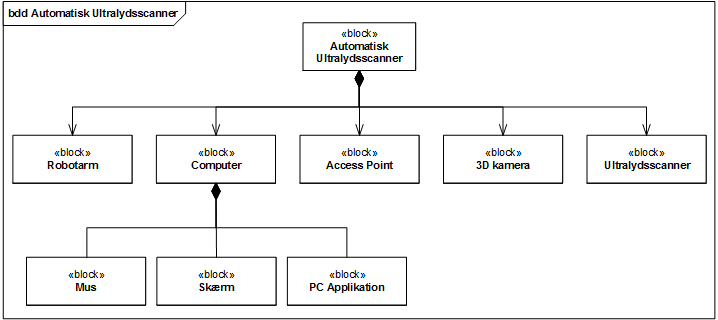
\includegraphics[width=1\textwidth]{figurer/d/Design/BDD}
    \caption{BDD for Automatisk Ultralydsscanner}
    \label{BDD}
\end{figure}

\section{Internal block diagram}
Internal block diagram Figur \ref{IBD} viser systemets interne forbindelser og flow mellem de forskellige blokke. Her er ultralydsscanner ikke er inkluderet, da den ikke har forbindelse til de andre blokke udover at være fysisk monteret på robotarm. 

\begin{figure}[H]
    \centering
    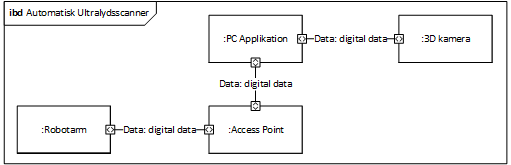
\includegraphics[width=1\textwidth]{figurer/d/Design/IBD}
    \caption{IBD for Automatisk Ultralydsscanner}
    \label{IBD}
\end{figure}

\section{Systemets grænseflader}